\documentclass{amsart}

\usepackage[english]{babel}
\usepackage[utf8]{inputenc}
\usepackage{graphicx}
\usepackage{mathtools}
\usepackage{amsthm}
\usepackage{amsfonts}
\usepackage{hyperref}
\usepackage[singlelinecheck=false]{caption}
\usepackage[backend=biber,url=true,doi=true,eprint=false,style=alphabetic]{biblatex}
\usepackage{enumitem}
\usepackage[justification=centering]{caption}
\usepackage{indentfirst}
\usepackage{algorithm}
\usepackage{algpseudocode}

\addbibresource{references.bib}

\makeatletter
\def\subsection{\@startsection{subsection}{3}%
  \z@{.5\linespacing\@plus.7\linespacing}{.1\linespacing}%
  {\normalfont\itshape}}
\makeatother

\DeclareMathOperator*{\argmin}{arg\,min}
\DeclareMathOperator*{\argmax}{arg\,max}

\newcommand\defeq{\mathrel{\overset{\makebox[0pt]{\mbox{\normalfont\tiny\sffamily def}}}{=}}}

\algrenewcommand\algorithmicrequire{\textbf{Input}}
\algrenewcommand\algorithmicensure{\textbf{Output}}

\captionsetup[table]{labelsep=space}

\theoremstyle{plain}

\newtheorem*{definition}{Definition}
\newtheorem{theorem}{Theorem}
\newtheorem{proposition}{Proposition}

\newcommand{\set}[1]{\mathcal{#1}}
\newcommand{\pr}{\mathbb{P}}
\renewcommand{\implies}{\Rightarrow}

\setlength{\parskip}{1em}

\title[]{3. Independencies}
\author[]{Renato Lui Geh\\NUSP\@: 8536030}

\begin{document}

\begin{abstract}
  This document shows how to represent independencies in bayesian networks. We present ways to find
  and specify independencies in the network's DAG\@. We introduce semi-graphoids, graphoids,
  d-separation and m-separation formally. We then show how to apply d-separation and m-separation
  on the bayesian network to explore the DAG's variable independency properties. Finally we analyse
  the BayesBall algorithm proposed by Schachter~\cite{bayesball}.

  \vspace*{-2.5em}
\end{abstract}

\maketitle

\section{Graphoids and Semi-graphoids}

A graphoid follows a set of rules that define variable independence as sets of paths in a graph.

\begin{enumerate}
  \item Symmetry: $X\perp Y|Z\implies Y\perp X|Z$
  \item Decomposition: $X\perp Y\cup W|Z\implies X\perp Y|Z$
  \item Weak union: $X\perp Y\cup W|Z\implies X\perp Y|Z\cup W$
  \item Contraction: $X\perp W|Y\cup Z, X\perp Y|Z\implies X\perp Y\cup W|Z$
  \item Intersection: $X\perp Y|Z\cup W, X\perp W|Z\cup Y\implies X\perp Y\cup W|Z$ if $\pr>0$
\end{enumerate}

A dependency model $I(X,Z,Y)\equiv X\perp Y|Z$ is a graphoid iff it is closed under conditions
(i)--(v). A semi-graphoid is closed under (i)--(iv). Rule (v) only holds if the probability
function is positive. It was believed that these five rules were axiomatic rules that defined
independency accurately~\cite{graphoids-pearl}. However, Studeny later proved that semi-graphoids
cannot be used to specify independence exactly~\cite{graphoids-studeny}. In spite of that,
semi-graphoids continue to provide us with a set of useful properties to explore independency in
bayesian networks.

\section{Markov Properties}

In the previous document we had defined Markov Property as:

\begin{equation*}
  X\perp Nd(X) | Pa(X)
\end{equation*}

This property is also called Local Markov Property (LMP). Another important property that is
associated with LMP is the Ordered Markov Property (OMP):

\begin{equation*}
  X\perp \{Y:Y<X\} | Pa(X)\text{, where $<$ is a topological order.}
\end{equation*}

We can use Decomposition, from our previous section, to derive yet another property:

\begin{equation*}
  X\perp Y | Pa(X) \forall Y \in Nd(X)
\end{equation*}

This property is known as Pairwise Markov Property (PMP). We can derive PMP with Decomposition,
yet the other way around (through Composition) does not hold in general unless the distribution is
positive, in which case we may apply Intersection and the property holds.

\section{Trails, Paths and Connectivity of a Graph}

Let $G=(V,E)$ be a DAG\@. A trail is a sequence of nodes $X_1,\ldots,X_n$ in $V$ such that $(X_i,
X_{i+1})$ mutual exclusive or $(X_{i+1},X_i)$ is an arc in $E$ and appears only once. An arc is a
directed edge in $E$ that connects two nodes $(X,Y)$ such that $X\rightarrow Y$. The length of a
trail is the number of nodes a trail passes on. A directed path is a trail that follows the
direction of the arcs. A node $X$ is connected with another node $Y$ if there exists a trail
$X,\ldots,Y$. If there is no such trail, then $X$ and $Y$ are separated. A directed cycle is a
trail that starts and ends on the same node.

\section{D-separation}

A dependency graph is an acyclic and directed graph where its edges are dependencies. Take Figure 1
as example: $B$ \textit{depends} on $A$. This means that $A\not\perp B$. A dependency graph must
follow the properties defined for graphoids.

\begin{figure}[h]
  \captionsetup{justification=centering}
  \centering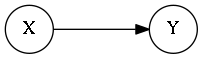
\includegraphics[scale=0.3]{graphs/dep.png}
  \caption{A dependency graph where nodes $X$ and $Y$ are probabilistically dependent. In this case
  we have that $X\perp Y$.}
\end{figure}

D-separation can be summarized into three categories in a dependency graph. The first case happens
when we have the following DAG\@:

\begin{figure}[h]
  \captionsetup{justification=centering}
  \centering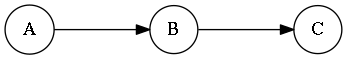
\includegraphics[scale=0.3]{graphs/serial.png}
  \caption{In a serial connection we have that $A\perp C|B$ and $A\not\perp C|\emptyset$.}
\end{figure}

This is called a \textit{serial connection}. Node $B$ \textit{blocks} nodes $A$ and $C$, meaning
$A$ and $C$ can only be independent of each other (i.e.\ no dependence edge) if $B$ is removed.
Thus, if we can say that $A\perp C|B$ and $A\not\perp C|\emptyset$. That is, if we remove $B$, we
have \textit{unblocked} $A$ and $C$ that were otherwise blocked by $B$. We say in this situation
that $A$ and $C$ are \textit{d-separated} by $B$.

The second case is known as a \textit{divergent connection}. It happens when a node has two edges
that directly connect two distinct other nodes. This can be read as $B$ being the common cause to
the effects $A$ and $B$.

\begin{figure}[h]
  \captionsetup{justification=centering}
  \centering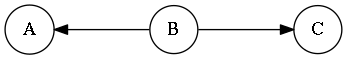
\includegraphics[scale=0.3]{graphs/divergent.png}
  \caption{In a divergent connection we have that $A\perp C|B$ and $A\not\perp C|\emptyset$.}
\end{figure}

Note that if we take into account what we have said earlier about serial connectivity, we can apply
the same concepts we used and derive the same conclusions. If we remove node $B$, we have that
$A$ and $C$ are now unblocked and are now independent $A\not\perp C|\emptyset$. Otherwise $B$
blocks $A$ and $C$ and so $A\perp C|B$. Therefore we can say that $A$ and $C$ are d-separated by
$B$.

The third and last case is called the \textit{convergent connection}. In this case we have $B$ as
the common effect of $A$ and $C$ (or $A$ and $C$ are the common causes of $B$). This is scenario is
known as \textit{explaining away}.

\begin{figure}[h]
  \captionsetup{justification=centering}
  \centering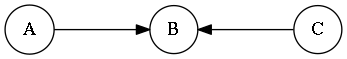
\includegraphics[scale=0.3]{graphs/convergent.png}
  \caption{In a convergent connection we have that $A\not\perp C|B$ and $A\perp C|\emptyset$.}
\end{figure}

In this case we have that the trail from $A$ to $C$ is unblocked when $B$ is not removed and
blocked otherwise. Node $A$ is independent of $C$ when we have no common effects, and dependent of
each other when they have a common effect. We say, in this case, that $A$ and $C$ are d-connected
by $B$. This might seem confusing at first, but take the following situation as example:

\begin{figure}[h]
  \captionsetup{justification=centering}
  \centering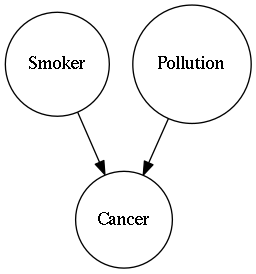
\includegraphics[scale=0.3]{graphs/cancer.png}
  \caption{$Smoker$ and $Pollution$ are initially independent of each other. However, if we know
  our patient has $Cancer$, we might alter the probabilities of our causes accordingly.}
\end{figure}

Consider the situation where we have a dependency graph that attributes $Smoker$ and $Pollution$ as
common causes to the effect $Cancer$. One could say that smoking and pollution are two independent
events (if we assume that smoking does not lead to pollution or that people that smoke are drawn to
polluted places), and that smoking and pollution cause cancer (again, we simplify our world to fit
our example). But suppose that our patient has cancer, then we can say that the probability of him
smoking or being in constant contact with pollution increases, since they are both possible causes
of cancer. If we then discover that our patient also smokes, this might lead to the decrease of our
belief that he has been in contact with pollution, since we have found a more probable cause to his
cancer. Notice that even though the two causes are independent of each other separately (i.e.\ if
we do not consider cancer), they have an direct influence on each other when one finds that the
common effect is known.

Let us now formally define what a blocked and unblocked trail is.

\begin{definition}
  A trail from $X$ to $Y$ is blocked by a set of nodes $\mathcal{B}$ if:
  \begin{enumerate}
    \item $X$ or $Y$ are in $\mathcal{B}$, or
    \item There exists a serial or divergent connection $X,Y,Z$ and $Y\in\mathcal{B}$, or
    \item There exists a convergent connection $X\rightarrow Y\leftarrow Z$ and $(\{Y\}\cup Nd(Y))
      \not\subseteq\mathcal{B}$, that is, neither $Y$ nor any of its descendants are in
      $\mathcal{B}$.
  \end{enumerate}
  Otherwise, the trail is unblocked.
\end{definition}

Now we define d-separation:

\begin{definition}
  Sets of nodes $\mathbf{X}$ and $\mathbf{Y}$ are d-separated by a set of nodes $\mathbf{Z}$ if
  every trail from a variable $X\in\mathbf{X}$ to a variable $Y\in\mathbf{Y}$ is blocked by $Z$.
  Otherwise, $\mathbf{X}$ and $\mathbf{Y}$ are d-connected. We will denote d-separation with the
  symbol $\perp_d$. Thus, if $\mathbf{X}$ and $\mathbf{Y}$ are d-separated by $\mathbf{Z}$:

  \begin{equation*}
    \mathbf{X} \perp_d \mathbf{Y} | \mathbf{Z}
  \end{equation*}
\end{definition}

An alternative way of denoting d-separation is through a function $D$ that takes three arguments
$\mathbf{X},\mathbf{Z},\mathbf{Y}$. Sets $\mathbf{X}$ and $\mathbf{Y}$ are d-separated from
$\mathbf{Z}$ if $D(X,Z,Y)$ is true. D-separation is consistent with LMP because of the following
proposition:

\begin{proposition}
  Any node $X$ is d-separated from its nondescendants by its parents.
\end{proposition}

Our objective is to equate d-separation with independency. For this we must require that
d-separation be both sound and complete.

\begin{description}
  \item[(1) Soundness] $\mathbf{X}\perp_d\mathbf{Y}|\mathbf{X}\implies\mathbf{X}\perp\mathbf{Y}|
    \mathbf{Z}$
  \item[(2) Completeness] $\mathbf{X}\perp\mathbf{Y}|\mathbf{X}\implies\mathbf{X}\perp_d\mathbf{Y}|
    \mathbf{X}$
\end{description}

We know that (1) holds.

\begin{theorem}\label{soundness}
  D-separation is sound.
\end{theorem}

Condition (1) is known as Global Markov Property (GMP). GMP implies LMP and LMP implies GMP\@. In
fact, we can take the following table as a good rule of thumb:

\begin{align*}
  &GMP \implies LMP \implies PMP\\
  &PMP \not\implies LMP \implies GMP
\end{align*}

However, d-separation is not complete for all distributions. We will now show a couple of important
theorems:

\begin{theorem}
  For any $G$ graph, there exists a Bayesian network with graph $G$ and variables $X$ and $Y$ such
  that $X\perp Y$ and $X\not\perp_d Y$.
\end{theorem}

\begin{theorem}
  If $G$ is a DAG and $X$ and $Y$ are d-connected by $Z$ in $G$, then there is a Bayesian network
  $(G,\pr)$ such that $X$ and $Y$ are dependent given $Z$.
\end{theorem}

\section{Markov's Blanket}

A Markov Blanket is defined as:

\begin{definition}
  The Markov blanket of a variable $X$ in a graph $G=(V,E)$ is the set $\mathcal{B}$ in which
  \begin{equation*}
    X\perp V\setminus\mathcal{B}\setminus\{X\}|\mathcal{B}
  \end{equation*}
\end{definition}

\begin{proposition} Exercise 1\\
  The set formed by the parents, the children and the parents of the children of a variable $X$ is
  a Markov blanket of $X$. If the distribution is positive it is minimal.
\end{proposition}

\begin{proof}
  We can summarize all possible outcomes a bayesian network may take with the following network:

  \begin{figure}[h]
    \captionsetup{justification=centering}
    \centering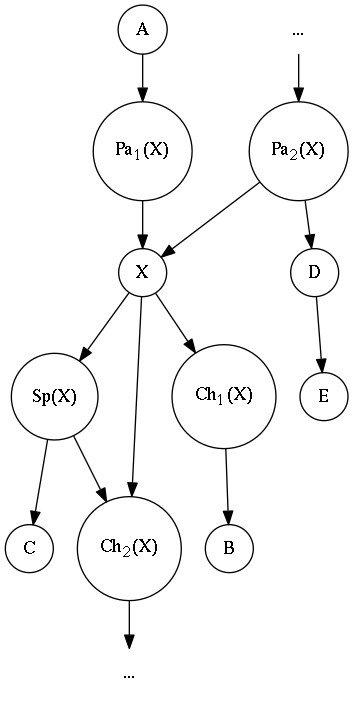
\includegraphics[scale=0.3]{graphs/markov_blanket.png}
    \caption{All possible connections with $X$ and other nodes outside of the Markov Blanket are
    either serial or divergent.}
  \end{figure}

  \begin{align*}
    &A\perp X|Pa(X)\\
    &B\perp X|Ch(X)\\
    &C\perp X|Sp(X)\\
    &D\perp X|Pa(X)\\
    &E\perp X|Pa(X)\\
  \end{align*}

  The set $Sp(X)$ are the set of spouses of $X$. That is, $Sp(X)=Pa(Ch(X))\setminus\{X\}$.

  From this bayesian network we can easily see that all possible connections from variable $X$ to
  or from another node is through a serial or divergent connection. Since a serial or divergent
  connection implies in $X\perp_d Y\not\in\mathcal{B}|\mathcal{B}$, we can extend this, from
  Theorem~\ref{soundness}, that it suffices to show that the markov blanket d-separates $X$ from
  any other node that is not in $\mathcal{B}$.
\end{proof}

D-separation satisfies all properties that define semi-graphoids and also composition and
intersection. However, since not all distributions satisfy these two last properties, there are
distributions that cannot be fully described by a bayesian network.

\section{M-separation}

M-separation verifies independency in an undirected graph.

\begin{definition}
  A moral graph of a DAG $G$ is the resulting undirected graph of, for every node $X$, connecting
  every $X$ to its respective $Sp(X)$ only once.
\end{definition}

\begin{definition}
  Sets of variables $\mathbf{X}$ and $\mathbf{Y}$ are m-separated by $\mathbf{Z}$ if $\mathbf{X}$
  and $\mathbf{Y}$ are separated in the moral graph associated with $(An(\mathbf{X})\cup
  An(\mathbf{Y})\cup An(\mathbf{Z}))\setminus \mathbf{Z}$.
\end{definition}

\begin{theorem}
  $\mathbf{X}\perp_d\mathbf{Y}|\mathbf{Z} iff \mathbf{X}\perp_m\mathbf{Y}|\mathbf{Z}$, where
  $\perp_m$ denotes m-separation.
\end{theorem}

\newpage

\printbibliography[]

\end{document}
